\documentclass[11pt,aspectratio=43]{beamer}

\usepackage{amsmath,amssymb}
\usepackage{booktabs}
\usepackage{graphicx}
\usepackage{xcolor}
\usepackage{tikz}
\usetikzlibrary{arrows.meta,positioning,shapes.geometric,calc}

\definecolor{accent}{HTML}{2E75B6}
\definecolor{red2}{HTML}{C0392B}
\definecolor{green2}{HTML}{27AE60}
\definecolor{orange2}{HTML}{E67E22}

\setbeameroption{hide notes}
\setbeamertemplate{navigation symbols}{}
\setbeamersize{text margin left=0.9cm,text margin right=0.9cm}

\setbeamercolor{normal text}{fg=black,bg=white}
\setbeamercolor{frametitle}{fg=black,bg=white}
\setbeamercolor{title}{fg=black}
\setbeamercolor{structure}{fg=black}
\setbeamercolor{alerted text}{fg=accent}
\setbeamercolor{block title}{fg=black,bg=black!10}
\setbeamercolor{block body}{fg=black,bg=black!3}
\setbeamercolor{itemize item}{fg=black}
\setbeamercolor{itemize subitem}{fg=black}

\setbeamerfont{title}{size=\normalsize,series=\bfseries}
\setbeamerfont{frametitle}{size=\normalsize,series=\bfseries}
\setbeamerfont{block title}{size=\small,series=\bfseries}
\setbeamerfont{block body}{size=\small}

\setbeamertemplate{footline}{%
  \leavevmode%
  \hbox{%
    \begin{beamercolorbox}[wd=\paperwidth,ht=2.5ex,dp=1.0ex,rightskip=0.9cm]{author in head/foot}%
      \hfill\insertframenumber
    \end{beamercolorbox}%
  }%
}

\title{Octopus CXL Memory Pooling:\\RL Results, Training System, and Next Steps}
\author{Pulak Mehrotra}
\date{April 2026}

\begin{document}

\begin{frame}[plain]
  \titlepage
\end{frame}

% =========================================================================
% SLIDE 1 — Three takeaways
% =========================================================================

\begin{frame}{Three takeaways.}

  \vspace{0.4em}

  \begin{enumerate}
    \setlength{\itemsep}{1.5em}

    \item \textbf{RL is the only policy near break-even on both held-out traces.}\\[0.2em]
          Greedy fails on both traces (ratio 3.77 and 12.97).
          RL achieves pooling ratio 0.98 and 1.06 --- at or below break-even.

    \item \textbf{The training system is not the bottleneck.}\\[0.2em]
          Data augmentation across 7 traces and 32 parallel environments
          solved generalisation and eliminated policy collapse.

    \item \textbf{The remaining ceiling is a reward design problem.}\\[0.2em]
          Savings plateau at $\sim$1--2\% within 100k steps and do not
          improve over 2M steps.
          The agent learns to game the proxy reward rather than
          maximise true pooling savings.

  \end{enumerate}

\end{frame}

% =========================================================================
% SLIDE 2 — Bar chart + takeaways
% =========================================================================

\begin{frame}{RL is the only policy near break-even on both held-out traces.}

  \begin{columns}[T,onlytextwidth]

    \column{0.62\textwidth}
      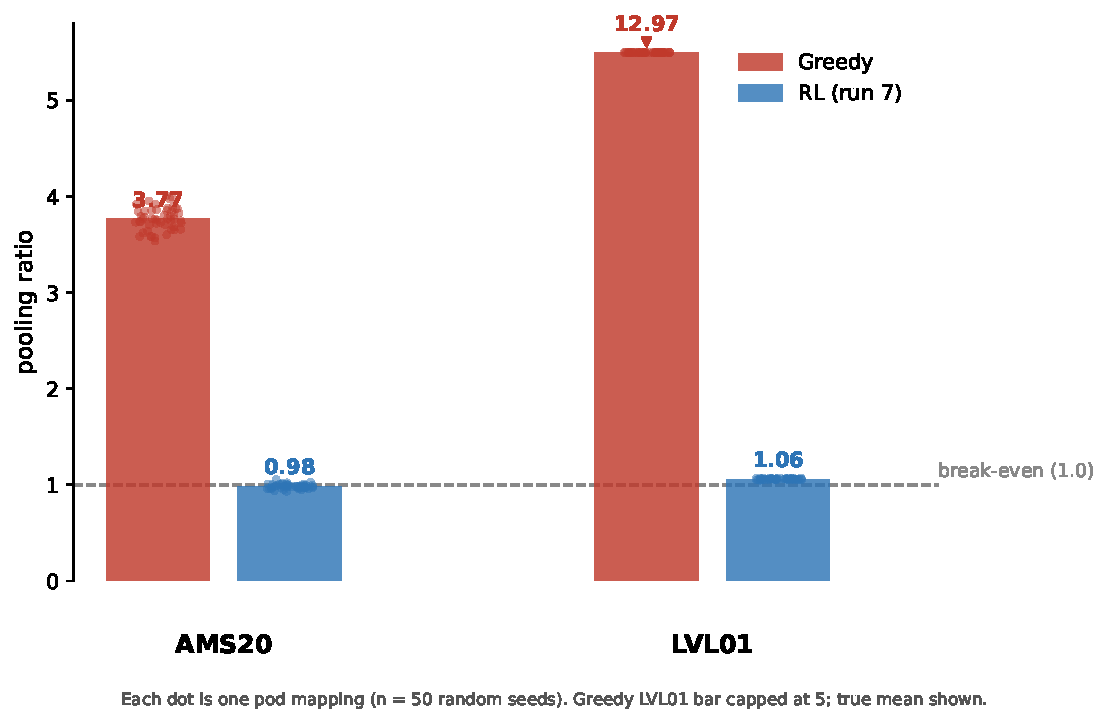
\includegraphics[width=\linewidth]{comparison_bar.pdf}

    \column{0.38\textwidth}
      \vspace{1.2em}
      \begin{itemize}
        \setlength{\itemsep}{1.0em}
        \item Both test traces were \textbf{unseen during training}.
        \item Dots show all 50 pod mappings --- results are \textbf{stable}.
        \item $n{=}50$ random pod mappings at 100\% CXL fraction (production $\approx$65\%).
      \end{itemize}

  \end{columns}

\end{frame}

% =========================================================================
% SLIDE 3 — MPD timeseries: greedy vs RL
% =========================================================================

\begin{frame}{Greedy packs load onto a few MPDs; RL spreads it.}

  \begin{columns}[T,onlytextwidth]

    \column{0.50\textwidth}
      \begin{center}
      \textbf{Greedy} \hfill \textcolor{red2}{pooling ratio $\approx$ 6.1}

      \vspace{0.2em}
      \includegraphics[width=\linewidth]{%
        ../../../../output/plots/memory_pooling/%
        LON23PrdApp01-troundgrt5m.sqlite_mhd_timeseries_greedy_pct0.5_pod16.png}

      \vspace{0.1em}
      \small A few MPDs saturate; most stay idle.
      \end{center}

    \column{0.50\textwidth}
      \begin{center}
      \textbf{RL (run 7)} \hfill \textcolor{accent}{pooling ratio $\approx$ 1.04}

      \vspace{0.2em}
      \includegraphics[width=\linewidth]{%
        ../../../../output/plots/memory_pooling/%
        LON23PrdApp01-troundgrt5m.sqlite_mhd_timeseries_rl_pct0.5_pod16.png}

      \vspace{0.1em}
      \small Load spread across all MPDs; no bottleneck.
      \end{center}

  \end{columns}

  \vspace{0.2em}
  \begin{center}
    \small\textit{LON23 (validation trace), CXL fraction 0.5, pod of 16 nodes.
    Each line = one MPD's load over time.}
  \end{center}

\end{frame}

% =========================================================================
% SLIDE 4 — Data augmentation: before vs after
% =========================================================================

\begin{frame}{Data augmentation solved generalisation.}

\begin{columns}[T,onlytextwidth]

% ── BEFORE ──────────────────────────────────────────────────────────
\column{0.34\textwidth}
  \begin{center}
  \textbf{Before}
  \vspace{0.4em}

  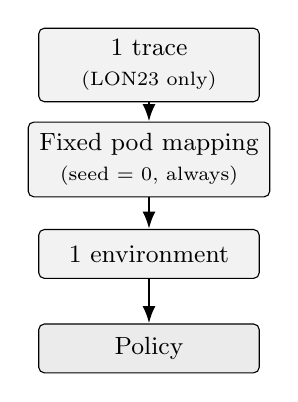
\begin{tikzpicture}[
    box/.style={draw, rounded corners=2pt, fill=black!5,
                minimum width=2.8cm, minimum height=0.62cm,
                align=center, font=\small, inner sep=4pt},
    arr/.style={-{Latex[length=2.2mm]}, line width=0.9pt},
  ]
    \node[box] (tr)  at (0, 3.6) {1 trace \\ \scriptsize(LON23 only)};
    \node[box] (map) at (0, 2.4) {Fixed pod mapping \\ \scriptsize(seed = 0, always)};
    \node[box] (env) at (0, 1.2) {1 environment};
    \node[box, fill=black!8] (pol) at (0, 0.0) {Policy};
    \draw[arr] (tr)  -- (map);
    \draw[arr] (map) -- (env);
    \draw[arr] (env) -- (pol);
  \end{tikzpicture}

  \vspace{0.4em}
  \small\textcolor{red2}{Memorises one DC.\\Fails on new traces.}
  \end{center}

% ── AFTER ───────────────────────────────────────────────────────────
\column{0.66\textwidth}
  \begin{center}
  \textbf{After}
  \vspace{0.4em}

  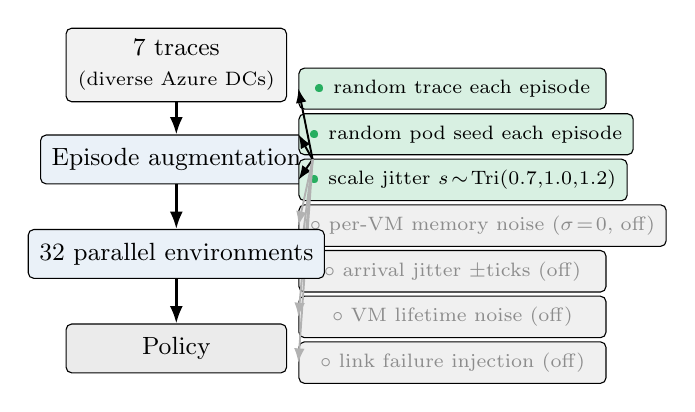
\begin{tikzpicture}[
    box/.style={draw, rounded corners=2pt, fill=black!5,
                minimum width=2.8cm, minimum height=0.62cm,
                align=center, font=\small, inner sep=4pt},
    kon/.style={draw, rounded corners=2pt, fill=green2!18,
                minimum width=3.9cm, minimum height=0.52cm,
                align=left, font=\scriptsize, inner sep=4pt},
    koff/.style={draw, rounded corners=2pt, fill=black!6,
                 minimum width=3.9cm, minimum height=0.52cm,
                 align=left, font=\scriptsize, inner sep=4pt,
                 text=black!45},
    arr/.style={-{Latex[length=2.2mm]}, line width=0.9pt},
    karr/.style={-{Latex[length=1.8mm]}, line width=0.7pt},
  ]
    \node[box] (tr) at (0, 3.6)
      {7 traces \\ \scriptsize(diverse Azure DCs)};

    \node[box, fill=accent!10] (aug) at (0, 2.4)
      {Episode augmentation};

    % Active knobs (green)
    \node[kon, anchor=west] (k1) at (1.55, 3.30)
      {\textcolor{green2}{\textbullet}~random trace each episode};
    \node[kon, anchor=west] (k2) at (1.55, 2.72)
      {\textcolor{green2}{\textbullet}~random pod seed each episode};
    \node[kon, anchor=west] (k3) at (1.55, 2.14)
      {\textcolor{green2}{\textbullet}~scale jitter $s\!\sim\!\mathrm{Tri}(0.7,\!1.0,\!1.2)$};

    % Disabled knobs (grey)
    \node[koff, anchor=west] (k4) at (1.55, 1.56)
      {$\circ$~per-VM memory noise ($\sigma\!=\!0$, off)};
    \node[koff, anchor=west] (k5) at (1.55, 0.98)
      {$\circ$~arrival jitter $\pm$ticks (off)};
    \node[koff, anchor=west] (k6) at (1.55, 0.40)
      {$\circ$~VM lifetime noise (off)};
    \node[koff, anchor=west] (k7) at (1.55,-0.18)
      {$\circ$~link failure injection (off)};

    \draw[karr] (aug.east) -- (k1.west);
    \draw[karr] (aug.east) -- (k2.west);
    \draw[karr] (aug.east) -- (k3.west);
    \draw[karr, black!30] (aug.east) -- (k4.west);
    \draw[karr, black!30] (aug.east) -- (k5.west);
    \draw[karr, black!30] (aug.east) -- (k6.west);
    \draw[karr, black!30] (aug.east) -- (k7.west);

    \node[box, fill=accent!10] (env) at (0, 1.2)
      {32 parallel environments};
    \node[box, fill=black!8] (pol) at (0, 0.0) {Policy};

    \draw[arr] (tr)  -- (aug);
    \draw[arr] (aug) -- (env);
    \draw[arr] (env) -- (pol);
  \end{tikzpicture}

  \vspace{0.4em}
  \small\textcolor{green2}{Generalises to AMS20 \& LVL01 (never seen in training).}
  \end{center}

\end{columns}

\end{frame}

% =========================================================================
% SLIDE 5 — Parallel environments and training pipeline
% =========================================================================

\begin{frame}[shrink=5]{32 parallel environments cut rollout time by 26$\times$.}

  \begin{columns}[T,onlytextwidth]

    \column{0.40\textwidth}

      \vspace{0.2em}
      \textbf{Throughput}
      \begin{itemize}
        \setlength{\itemsep}{0.4em}
        \item Bottleneck: CPU rollout, not GPU.
        \item \texttt{DummyVecEnv(1)}: 46 steps/s
        \item \texttt{SubprocVecEnv(32)}: 1{,}221 steps/s
        \item \textbf{26$\times$ speedup.}
        \item 2M steps $\approx$ 14 min wall-clock.
      \end{itemize}

      \vspace{0.5em}
      \textbf{SAC hyperparameters}
      \begin{itemize}
        \setlength{\itemsep}{0.3em}
        \item $\gamma = 0.999$, replay 1M, batch 256
        \item $\alpha$ auto-tuned
        \item Net: $[256,\,256]$
      \end{itemize}

    \column{0.60\textwidth}
      \begin{center}
      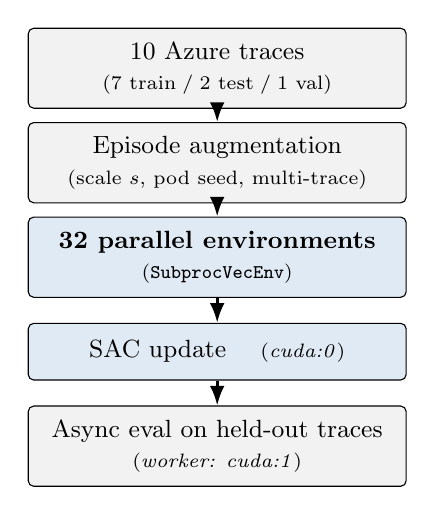
\begin{tikzpicture}[
          every node/.style={font=\small},
          box/.style={draw, rounded corners=2pt, fill=black!5,
                      minimum height=0.72cm, minimum width=4.8cm,
                      align=center, inner sep=5pt},
          arr/.style={-{Latex[length=2.5mm]}, line width=1.0pt}
      ]
        \node[box] (traces) at (0, 3.6)
              {10 Azure traces \\ \scriptsize(7 train\;/\;2 test\;/\;1 val)};

        \node[box] (aug) at (0, 2.4)
              {Episode augmentation \\ \scriptsize(scale $s$, pod seed, multi-trace)};

        \node[box, fill=accent!15] (envs) at (0, 1.2)
              {\textbf{32 parallel environments} \\ \scriptsize(\texttt{SubprocVecEnv})};

        \node[box, fill=accent!15] (sac) at (0, 0.0)
              {SAC update \quad \scriptsize(\textit{cuda:0})};

        \node[box] (eval) at (0,-1.2)
              {Async eval on held-out traces \\ \scriptsize(\textit{worker: cuda:1})};

        \draw[arr] (traces) -- (aug);
        \draw[arr] (aug)    -- (envs);
        \draw[arr] (envs)   -- (sac);
        \draw[arr] (sac)    -- (eval);
      \end{tikzpicture}
      \end{center}

  \end{columns}

\end{frame}

% =========================================================================
% SLIDE 6 — Reward design failure
% =========================================================================

\begin{frame}{The reward told the agent the wrong thing.}

  \begin{columns}[T,onlytextwidth]

    \column{0.58\textwidth}
      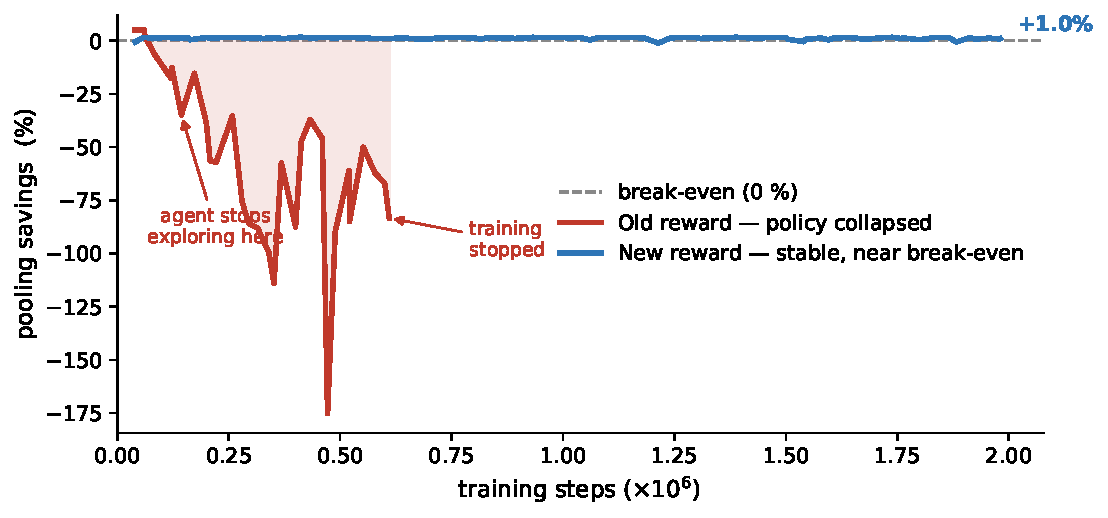
\includegraphics[width=\linewidth]{run6_vs_run7.pdf}

    \column{0.42\textwidth}
      \vspace{0.8em}

      \textbf{What went wrong}
      \begin{itemize}
        \setlength{\itemsep}{0.7em}
        \item The reward only watched the \textbf{single most-loaded MPD}.
        \item The agent found a shortcut: stop exploring and repeat one
              safe assignment.
        \item Pooling gets \textbf{worse}, not better.
      \end{itemize}

  \end{columns}

\end{frame}

% =========================================================================
% SLIDE 7 — Redesigned reward
% =========================================================================

\begin{frame}{Fix: score all MPDs, and discount VMs that are about to leave.}

  \begin{columns}[T,onlytextwidth]

    \column{0.50\textwidth}
      \vspace{0.3em}
      \textbf{Two changes to the reward}
      \begin{enumerate}
        \setlength{\itemsep}{0.8em}
        \item \textbf{Score all reachable MPDs} every step, not just the worst one.
              Every MPD now gives the agent feedback.
        \item \textbf{Discount short-lived VMs.}
              A VM leaving in 1\,hr should barely count against an MPD's load.
              A VM staying 2\,days should count fully.
      \end{enumerate}

      \vspace{0.9em}
      \textbf{Result:} stable training over 2M steps,
      near break-even on both held-out traces.

    \column{0.50\textwidth}
      \vspace{0.3em}
      \begin{center}
      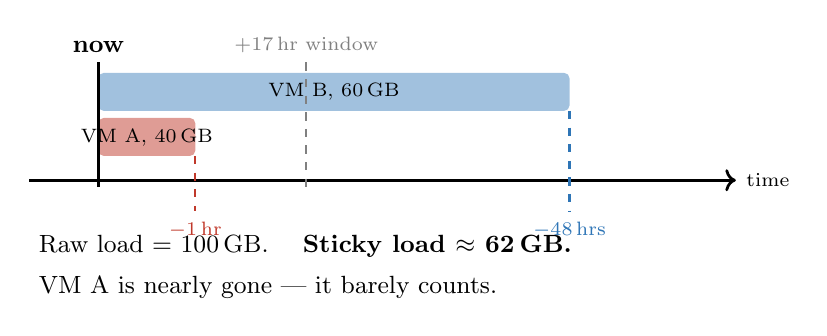
\begin{tikzpicture}[every node/.style={font=\small}, scale=0.88]
        \draw[->,line width=1pt] (0,0) -- (10.2,0)
          node[right,font=\scriptsize]{time};

        % VM A: departs in 1 hr
        \fill[red2!50,rounded corners=2pt] (1.0,0.35) rectangle (2.4,0.9);
        \node[font=\scriptsize] at (1.7,0.62) {VM A, 40\,GB};
        \draw[red2,dashed,line width=0.8pt] (2.4,0.35) -- (2.4,-0.45)
          node[below,font=\scriptsize,red2] {$-$1\,hr};

        % VM B: stays
        \fill[accent!45,rounded corners=2pt] (1.0,1.0) rectangle (7.8,1.55);
        \node[font=\scriptsize] at (4.4,1.27) {VM B, 60\,GB};
        \draw[accent,dashed,line width=0.8pt] (7.8,1.0) -- (7.8,-0.45)
          node[below,font=\scriptsize,accent] {$-$48\,hrs};

        % Now marker
        \draw[black,line width=1.3pt] (1.0,1.7) -- (1.0,-0.1);
        \node[above,font=\small\bfseries] at (1.0,1.7) {now};

        % 17-hr window
        \draw[dashed,gray,line width=0.8pt] (4.0,1.7) -- (4.0,-0.1);
        \node[above,font=\scriptsize,gray] at (4.0,1.7) {$+$17\,hr window};

        \node[font=\small,align=left,anchor=west] at (0.0,-0.95)
          {Raw load = 100\,GB. \quad\textbf{Sticky load $\approx$ 62\,GB.}};
        \node[font=\small,align=left,anchor=west] at (0.0,-1.55)
          {VM~A is nearly gone --- it barely counts.};
      \end{tikzpicture}
      \end{center}

  \end{columns}

\end{frame}

% =========================================================================
% SLIDE 8 — Savings plateau
% =========================================================================

\begin{frame}[shrink=8]{The new reward is stable --- but stuck at 1--2\%.}

  \begin{columns}[T,onlytextwidth]

    \column{0.62\textwidth}
      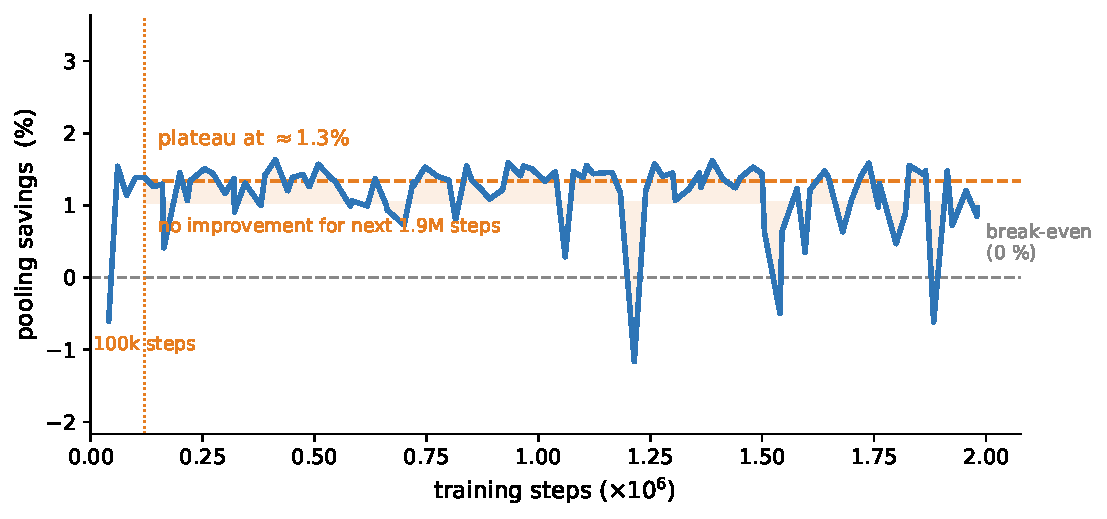
\includegraphics[width=\linewidth]{plateau.pdf}

    \column{0.38\textwidth}
      \vspace{1.0em}
      \begin{itemize}
        \setlength{\itemsep}{1.1em}
        \item Savings reach $\approx$1--2\% within 100k steps, then \textbf{stop improving}.
        \item Training for 20$\times$ longer changes nothing.
        \item \textbf{More training is not the fix.}
              The agent has learned to game the reward signal, not to maximise real savings.
      \end{itemize}

      \vspace{1.0em}
      \small The next slides explain why, and what reward changes we plan to try.

  \end{columns}

\end{frame}

% =========================================================================
% SLIDE 9 — Reward hacking
% =========================================================================

% =========================================================================
% SLIDE 9 — Why the agent is stuck: reward hacking
% =========================================================================

\begin{frame}[shrink=6]{The current reward is better --- but it still misses the big picture.}

  \begin{columns}[T,onlytextwidth]

    \column{0.50\textwidth}
      \vspace{0.3em}
      \small
      \begin{itemize}
        \setlength{\itemsep}{0.55em}
        \item \textbf{What the current reward does:} it gives a better score when a
              host avoids leaving a lot of long-lasting load on the MPDs it can use.
        \item \textbf{Why that helped:} this removed the collapse from the old reward
              and made training much more stable.
        \item \textbf{What it still misses:} it judges each host's choice mostly
              by looking at that host's own neighborhood.
        \item So a host can make its own score look better by splitting load
              evenly, even if that sends more traffic onto an MPD that is already
              crowded for the whole pod.
        \item The agent is improving the \emph{measured reward}, but not the real
              outcome we care about: \textbf{final pooling savings}.
      \end{itemize}

    \column{0.50\textwidth}
      \begin{center}
      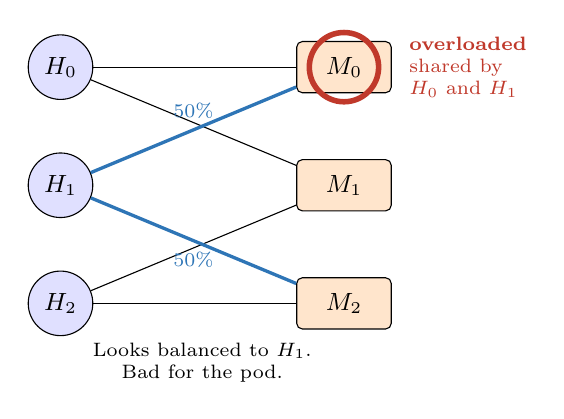
\begin{tikzpicture}[
          every node/.style={font=\small},
          host/.style={draw,circle,fill=blue!12,minimum size=0.82cm},
          mpd/.style={draw,rounded corners=2pt,fill=orange!20,
                      minimum width=1.2cm,minimum height=0.65cm,
                      align=center,font=\small},
      ]
        \node[host] (h0) at (0,3.0) {$H_0$};
        \node[host] (h1) at (0,1.5) {$H_1$};
        \node[host] (h2) at (0,0.0) {$H_2$};

        \node[mpd] (p0) at (3.6,3.0) {$M_0$};
        \node[mpd] (p1) at (3.6,1.5) {$M_1$};
        \node[mpd] (p2) at (3.6,0.0) {$M_2$};

        \draw (h0) -- (p0); \draw (h0) -- (p1);
        \draw (h1) -- (p0); \draw (h1) -- (p2);
        \draw (h2) -- (p1); \draw (h2) -- (p2);

        % H1 splits evenly (agent's choice)
        \draw[accent,very thick] (h1) -- (p0)
          node[midway,above,font=\scriptsize,accent] {50\%};
        \draw[accent,very thick] (h1) -- (p2)
          node[midway,below,font=\scriptsize,accent] {50\%};

        % M0 is the bottleneck
        \draw[red2,line width=2pt] (p0) circle (0.44cm);
        \node[red2,font=\scriptsize,align=left,right=0.1cm of p0]
          {\textbf{overloaded}\\shared by\\$H_0$ and $H_1$};

        \node[font=\scriptsize,align=center] at (1.8,-0.75)
          {Looks balanced to $H_1$.\\Bad for the pod.};
      \end{tikzpicture}
      \end{center}
  \end{columns}

\end{frame}

% =========================================================================
% SLIDE 10 — Reward-hacking fixes
% =========================================================================

\begin{frame}{What should the reward say instead?}

  \vspace{0.5em}

  \begin{itemize}
    \setlength{\itemsep}{1.1em}
    \item Score the agent on the \textbf{whole pod outcome}, not just whether one
          host made a locally good-looking choice; use \textbf{final pooling savings}
          as the main objective.
    \item Keep a small amount of step-by-step guidance with
          \textbf{potential-based reward shaping (PBRS)} so learning is easier,
          but the goal stays the same.
    \item Add an \textbf{optimal-gap} signal from the exact solver:
          tell the agent how far each placement is from the best possible choice
          for that snapshot.
  \end{itemize}

\end{frame}

\end{document}
